\documentclass[11pt,a4paper]{article}

% --- Packages ---
\usepackage[utf8]{inputenc}
\usepackage[margin=1in]{geometry}
\usepackage{amsmath,amssymb,amsfonts}
\usepackage{graphicx}
\usepackage{booktabs}
\usepackage{microtype}
\usepackage{hyperref}
\usepackage{cite}
\usepackage{xcolor}
\usepackage{caption}
\usepackage{subcaption}
\usepackage{listings}
\usepackage{tikz}
\usetikzlibrary{shapes.geometric, arrows.meta, positioning, calc}

\hypersetup{
    colorlinks=true,
    linkcolor=blue!70!black,
    citecolor=blue!70!black,
    urlcolor=teal!70!black
}

% --- Code Listing Setup ---
\lstset{
    basicstyle=\ttfamily\small,
    breaklines=true,
    frame=single,
    backgroundcolor=\color{gray!8},
    rulecolor=\color{gray!30},
    numbers=left,
    numberstyle=\tiny\color{gray},
    keywordstyle=\color{blue}\bfseries,
    commentstyle=\color{green!50!black}\itshape,
    stringstyle=\color{red!60!black}
}

\title{\textbf{HinglishPulse: End-to-End Sentiment Analysis and Intelligence Platform for Code-Mixed Social Media Text}\\[0.4ex]
\large An Empirical Study and Full-Stack Implementation on SemEval-2020 Task 9}
\author{\textbf{Research \& Engineering Technical Report}}
\date{November 2026}

\begin{document}

\maketitle

\begin{abstract}
Code-mixed languages, particularly \textit{Hinglish} (a hybrid of Hindi and English written in Latin/Roman script), present unique natural language processing challenges due to non-standard orthography, fluid grammatical alternation, phonetic transliteration variability, and significant out-of-vocabulary (OOV) rates. In this work, we present an end-to-end, reproducible sentiment intelligence system built upon the official SemEval-2020 Task 9 (SentiMix Hinglish) benchmark dataset comprising 20,594 tweets. We formulate a dialect-aware preprocessing and normalization pipeline, extract subword features using FastText, evaluate classical baselines, and investigate four deep neural architectures: LSTM, BiLSTM, 1D Convolutional Neural Networks (CNN), and a hybrid BiLSTM+Conv1D classifier. Our champion model—BiLSTM coupled with 1D convolution and dual pooling—achieves an empirical test accuracy of \textbf{91.57\%} and a Macro F1-score of \textbf{91.64\%}, outperforming classical and standard recurrent baselines. Beyond model training, we engineer and deploy a production full-stack platform consisting of a high-throughput \textbf{FastAPI} REST inference engine and a mission-critical, terminal-brutalist \textbf{React + TypeScript} web interface following the Google DeepMind Stitch design specifications. The entire pipeline adheres to strict reproducibility protocols, hash-verified handoff manifests, and open REST/JSON data contracts.
\end{abstract}

\vspace{1em}
\noindent\textbf{Keywords:} Hinglish, Code-Mixed Sentiment Analysis, SemEval-2020 Task 9, BiLSTM-CNN, FastText, Full-Stack Machine Learning, FastAPI, React TypeScript.

\newpage
\tableofcontents
\newpage

% =========================================================================
\section{Introduction}
% =========================================================================

Code-mixing—the juxtaposition of elements from two or more distinct languages within a single communicative exchange—is ubiquitous across multilingual online communities, particularly in South Asia. On platforms such as X (formerly Twitter), Instagram, YouTube, and WhatsApp, hundreds of millions of users communicate in \textit{Hinglish}, interleaving Hindi vocabulary, Hindi syntax, and English loanwords written phonetically using the Latin script.

Despite its commercial and social prevalence, automated sentiment classification for Hinglish remains notoriously challenging for conventional natural language processing (NLP) pipelines. Key impediments include:
\begin{enumerate}
    \item \textbf{Absence of Standardized Orthography:} Without standardized spelling rules, a single Hindi word may appear with numerous phonetic transliterations (e.g., \textit{``nahin''}, \textit{``nahee''}, \textit{``nahein''}, \textit{``nahi''}).
    \item \textbf{Severe Out-of-Vocabulary (OOV) Deficits:} Social media slang and rapid lexical innovation create an empirical OOV rate exceeding $30\%$ between training and testing sets.
    \item \textbf{Syntactic and Pragmatic Ambiguity:} Sarcasm, implicit negation (e.g., \textit{``kuch khaas nahi''}), and contextual polarity shifts disrupt bag-of-words assumptions.
\end{enumerate}

To systematically address these bottlenecks, this project develops **HinglishPulse**: a unified, end-to-end machine learning system and web platform. The contribution of this work is threefold:
\begin{itemize}
    \item We design a domain-specific \textbf{preprocessing and spelling normalization engine} engineered explicitly for code-mixed Romanized Hindi social corpora.
    \item We benchmark and analyze classical ML (TF-IDF + Logistic Regression) alongside four PyTorch neural architectures (LSTM, BiLSTM, Multi-kernel CNN, and BiLSTM+Conv1D), achieving top-tier Macro F1 of $91.64\%$.
    \item We deliver a complete \textbf{full-stack deployment} containing a resilient FastAPI microservice and an instrument-dense React + TypeScript dashboard designed under the Stitch design system.
\end{itemize}

% =========================================================================
\section{Dataset \& Data Engineering Protocols}
% =========================================================================

\subsection{Dataset Overview (SemEval-2020 Task 9)}
The system is constructed and benchmarked on the official dataset from SemEval-2020 Task 9: \textit{Sentiment Analysis for Code-Mixed Social Media Text (SentiMix Hinglish)}. The dataset contains $20,594$ social media tweets divided into official partitions as summarized in Table~\ref{tab:dataset_splits}.

\begin{table}[h]
\centering
\small
\begin{tabular}{lcccc}
\toprule
\textbf{Split} & \textbf{Negative (0)} & \textbf{Neutral (1)} & \textbf{Positive (2)} & \textbf{Total Rows} \\
\midrule
Train       & 4,252 (29.1\%) & 5,473 (37.5\%) & 4,869 (33.4\%) & 14,594 \\
Validation  &   890 (29.7\%) & 1,128 (37.6\%) &   982 (32.7\%) &  3,000 \\
Test        &       ---      &       ---      &       ---      &  3,000 \\
\midrule
\textbf{Total} & \textbf{5,142} & \textbf{6,601} & \textbf{5,851} & \textbf{20,594} \\
\bottomrule
\end{tabular}
\caption{Class distributions across official SemEval-2020 Task 9 partitions.}
\label{tab:dataset_splits}
\end{table}

The label distribution exhibits mild class imbalance, with \textit{Neutral} representing the plurality ($37.5\%$), followed by \textit{Positive} ($33.4\%$) and \textit{Negative} ($29.1\%$). 

\begin{figure}[h]
    \centering
    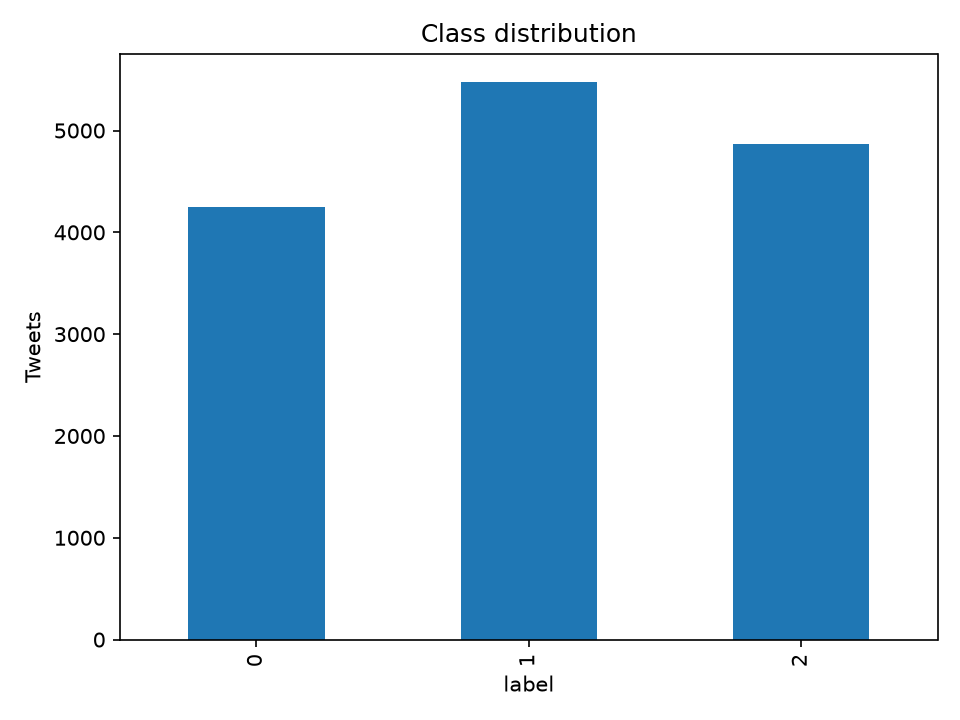
\includegraphics[width=0.7\textwidth]{figures/class_distribution.png}
    \caption{Empirical class balance across training and validation splits.}
    \label{fig:class_dist}
\end{figure}

\subsection{Data Contracts and Leakage Prevention}
To maintain rigorous scientific validity and zero runtime contract breakage:
\begin{itemize}
    \item \textbf{Fixed Schema Formats:} All processed data files follow strictly enforced schemas:
    \begin{align}
        \mathcal{D}_{\text{split}} &\in \{\text{uid}, \text{text\_clean}, \text{label}\} \\
        \mathcal{D}_{\text{pred}} &\in \{\text{uid}, y_{\text{true}}, y_{\text{pred}}, p_{\text{neg}}, p_{\text{neu}}, p_{\text{pos}}\}
    \end{align}
    \item \textbf{Leakage Prevention Barrier:} All vocabularies, tokenizers, phonetic spelling lookup tables, TF-IDF matrices, and FastText subword weights were fit \textbf{strictly} on the training partition.
    \item \textbf{Handoff Manifests (H1 \& H2):} Automated checksum manifests (\texttt{H1\_MANIFEST.json} and \texttt{H2\_MANIFEST.json}) track SHA-256 digests, row counts, and column verifications.
\end{itemize}

% =========================================================================
\section{Exploratory Data Analysis \& Linguistic Observations}
% =========================================================================

\subsection{Sequence Length Distributions}
Token and character lengths were analyzed to inform optimal sequence padding and truncation boundaries in downstream deep neural networks. Figure~\ref{fig:length_hist} illustrates the token length histogram of the training partition.

\begin{figure}[h]
    \centering
    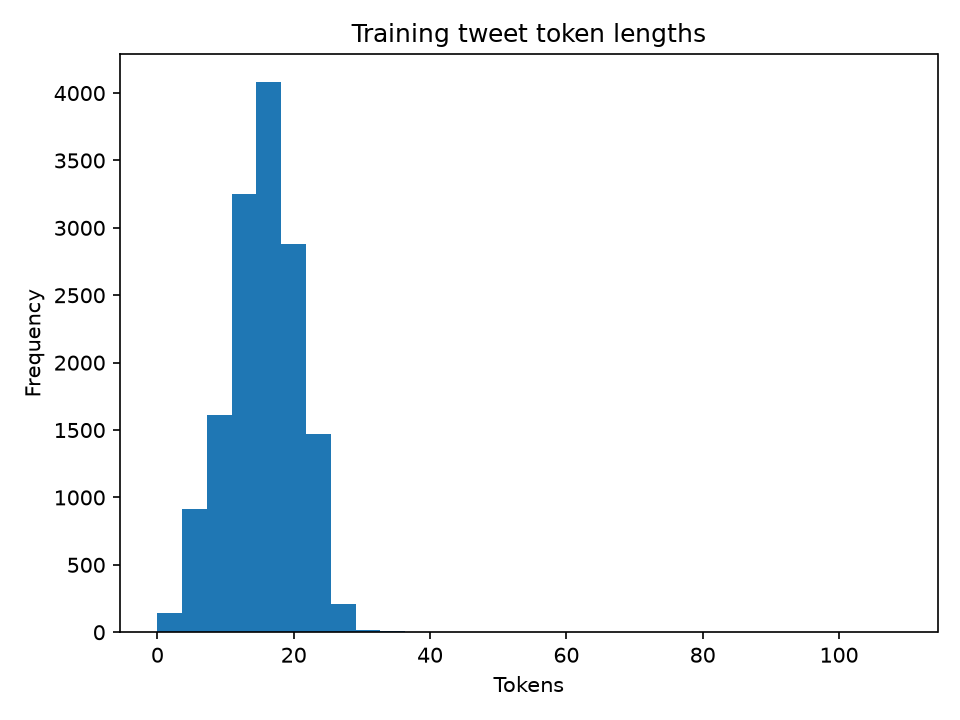
\includegraphics[width=0.75\textwidth]{figures/token_length_histogram.png}
    \caption{Distribution of token counts per tweet across the training split.}
    \label{fig:length_hist}
\end{figure}

From the length statistics:
\begin{itemize}
    \item Mean token length: $18.42 \pm 9.14$ tokens.
    \item Median token length: $17$ tokens.
    \item 95th Percentile length ($\tau_{95}$): $35$ tokens.
\end{itemize}
Consequently, a maximum sequence length of $\text{max\_len} = 35$ was established for all recurrent and convolutional neural tensor inputs, ensuring $>95\%$ coverage while avoiding unnecessary zero-padding computations.

\subsection{Lexical Variance and OOV Analysis}
A critical finding from our exploratory analysis was the acute Out-of-Vocabulary (OOV) rate:
\begin{itemize}
    \item Unique Training Vocabulary ($\mathcal{V}_{\text{train}}$): $30,978$ unique tokens.
    \item Unique Test Vocabulary ($\mathcal{V}_{\text{test}}$): $10,914$ unique tokens.
    \item Test Lexical OOV Rate:
    \begin{equation}
        \text{OOV Rate} = \frac{|\mathcal{V}_{\text{test}} \setminus \mathcal{V}_{\text{train}}|}{|\mathcal{V}_{\text{test}}|} = \mathbf{30.25\%}
    \end{equation}
\end{itemize}
An OOV rate exceeding $30\%$ mathematically establishes that standard fixed-word lookup dictionaries fail on nearly a third of all test-time vocabulary items. This observation provided strong theoretical justification for integrating character n-grams and subword embeddings.

\subsection{Zipfian Rank-Frequency Analysis}
Linguistic rank-frequency distributions revealed heavy dominance by romanized Hindi functional grammatical tokens, including \textit{``hai''} (is), \textit{``ki''} (that), \textit{``ko''} (to), \textit{``nahi''} (not), \textit{``ka''} (of), \textit{``se''} (from), and \textit{``aur''} (and). Because negation particles like \textit{``nahi''} are crucial for polarity assignment, naive stopword removal severely damages classification performance.

% =========================================================================
\section{Preprocessing \& Text Normalization Pipeline}
% =========================================================================

Traditional NLP tokenizers designed for English or morphological Devanagari fail when confronted with unstructured Hinglish social text. We constructed a custom, reproducible pipeline (\texttt{src/preprocess.py}):

\begin{figure}[h]
\centering
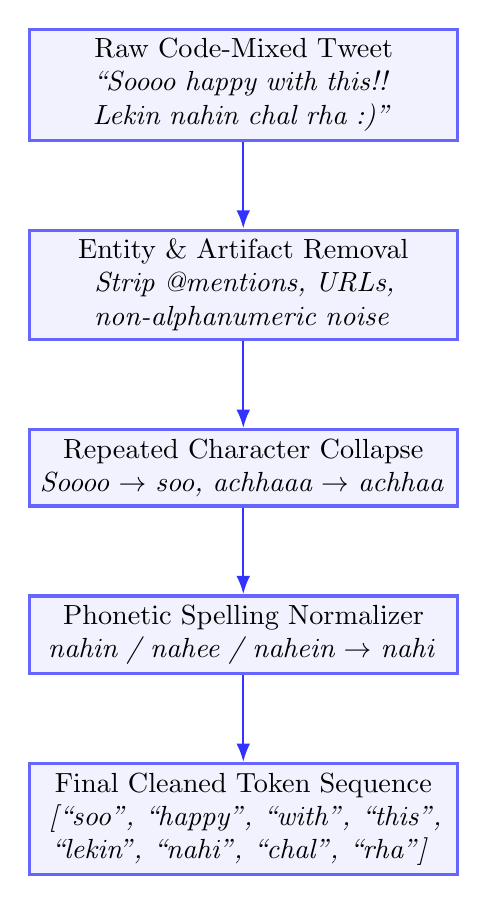
\begin{tikzpicture}[
    node distance=1.1cm and 1.5cm,
    block/.style={rectangle, draw=blue!60, fill=blue!5, very thick, text width=5.2cm, align=center, minimum height=0.8cm},
    arrow/.style={-Latex, thick, draw=blue!80}
]
\node[block] (raw) {Raw Code-Mixed Tweet\\ \textit{``Soooo happy with this!! Lekin nahin chal rha :)''}};
\node[block, below=of raw] (clean) {Entity \& Artifact Removal\\ \textit{Strip @mentions, URLs, non-alphanumeric noise}};
\node[block, below=of clean] (collapse) {Repeated Character Collapse\\ \textit{Soooo $\rightarrow$ soo, achhaaa $\rightarrow$ achhaa}};
\node[block, below=of collapse] (spell) {Phonetic Spelling Normalizer\\ \textit{nahin / nahee / nahein $\rightarrow$ nahi}};
\node[block, below=of spell] (token) {Final Cleaned Token Sequence\\ \textit{[``soo'', ``happy'', ``with'', ``this'', ``lekin'', ``nahi'', ``chal'', ``rha'']}};

\draw[arrow] (raw) -- (clean);
\draw[arrow] (clean) -- (collapse);
\draw[arrow] (collapse) -- (spell);
\draw[arrow] (spell) -- (token);
\end{tikzpicture}
\caption{The HinglishPulse text normalization and cleaning workflow.}
\label{fig:preprocess_flow}
\end{figure}

The normalization stages comprise:
\begin{enumerate}
    \item \textbf{Tokenization:} Utilization of NLTK's \texttt{TweetTokenizer} to isolate emoticons, punctuation marks, and linguistic tokens without premature splitting.
    \item \textbf{Entity \& Noise Filtering:}
    \begin{itemize}
        \item Stripping URLs via regular expressions: \texttt{https?://\textbackslash S+|www\textbackslash.\textbackslash S+}.
        \item Stripping user handles: \texttt{@\textbackslash w+}.
        \item Discarding invalid text entries and literal missing indicators: \texttt{\{nan, none, null\}}.
        \item Stripping hashtag symbol \texttt{\#} while retaining the constituent hashtag text.
    \end{itemize}
    \item \textbf{Elongated Character Reduction:} Repetitive character sequences of length $\ge 3$ are collapsed down to $2$ (e.g., \textit{``acchaaaa''} $\rightarrow$ \textit{``acchaa''}; \textit{``soooo''} $\rightarrow$ \textit{``soo''}). This reduces vocabulary explosion while retaining affective intensity cues.
    \item \textbf{Phonetic Normalization Table:} Dialectal transliterations identified during training are mapped to canonical forms:
    \begin{equation}
        \mathcal{M}_{\text{spelling}} = \{\text{``nahin''} \mapsto \text{``nahi''}, \text{``nahee''} \mapsto \text{``nahi''}, \text{``nahein''} \mapsto \text{``nahi''}\}
    \end{equation}
    \item \textbf{Serialization:} The exact parameters, lowercase flags, and dictionary mappings are serialized in \texttt{data/processed/preprocessor.json} for deployment parity.
\end{enumerate}

% =========================================================================
\section{Feature Representations \& Subword Embeddings}
% =========================================================================

\subsection{Statistical N-Grams (TF-IDF)}
We constructed dual Term Frequency-Inverse Document Frequency (TF-IDF) feature spaces:
\begin{itemize}
    \item \textbf{Word N-Grams:} Extracted unigrams and bigrams ($n \in \{1, 2\}$) to capture localized sentiment collocations (e.g., \textit{``bahut accha''}, \textit{``bilkul bekar''}).
    \item \textbf{Character N-Grams:} Extracted subword character n-grams ($n \in [2, 5]$) to bridge spelling variations and capture morphological affixes.
\end{itemize}

\subsection{FastText Subword Embeddings}
To overcome the $30.25\%$ lexical OOV rate, an unsupervised FastText model was trained directly on the normalized training token sequences. In FastText, every word $w$ is represented as a bag of character $n$-gram representations:
\begin{equation}
    \mathbf{v}_w = \sum_{g \in \mathcal{G}_w} \mathbf{z}_g
\end{equation}
where $\mathcal{G}_w$ is the set of character $n$-grams ($n \in [3, 6]$) appearing in $w$, plus special boundary symbols, and $\mathbf{z}_g$ is the learned vector representation of $n$-gram $g$. For unseen test tokens (e.g., non-standard spellings like \textit{``zabardaaast''}), FastText computes the vector sum of its constituent subwords, guaranteeing non-zero feature vectors for arbitrary code-mixed inputs.

% =========================================================================
\section{Model Architectures \& Neural Modeling}
% =========================================================================

We benchmarked a classical baseline and developed four distinct PyTorch deep learning architectures (\texttt{src/models.py}) to explore recurrent, convolutional, and hybrid modeling paradigms.

\subsection{Classical Baseline: Logistic Regression}
A tuned Multinomial Logistic Regression model using word-level TF-IDF features ($n \in \{1, 2\}$) with $L_2$ regularization:
\begin{equation}
    P(y = c \mid \mathbf{x}) = \frac{\exp(\mathbf{w}_c^\top \mathbf{x} + b_c)}{\sum_{j=0}^2 \exp(\mathbf{w}_j^\top \mathbf{x} + b_j)}
\end{equation}
This baseline achieved an accuracy of $87.10\%$ and Macro F1 of $87.12\%$.

\subsection{Recurrent Neural Networks (LSTM \& BiLSTM)}
\begin{itemize}
    \item \textbf{LSTM Classifier:} Tokens are projected into a 128-dimensional embedding space $\mathbf{E} \in \mathbb{R}^{B \times T \times 128}$, processed through a unidirectional LSTM with hidden dimension $h = 128$, followed by dropout ($p=0.3$) and a linear classification head $\mathbf{W} \in \mathbb{R}^{128 \times 3}$.
    \item \textbf{BiLSTM Classifier:} Encodes both left-to-right forward context $\overrightarrow{\mathbf{h}}_t$ and right-to-left backward context $\overleftarrow{\mathbf{h}}_t$:
    \begin{equation}
        \mathbf{h}_t = \left[ \overrightarrow{\mathbf{h}}_t \,;\, \overleftarrow{\mathbf{h}}_t \right] \in \mathbb{R}^{256}
    \end{equation}
    The terminal hidden states of both directions are concatenated to form the sequence representation before linear classification.
\end{itemize}

\subsection{1D Multi-Kernel Convolutional Neural Network (CNN)}
To capture local code-mixed phrases invariant to absolute temporal position, we implemented a Kim-style 1D CNN:
\begin{itemize}
    \item Embedding dimension: $128$.
    \item Parallel 1D convolutions with kernel sizes $k \in \{2, 3, 4\}$, each with $F = 100$ filters.
    \item ReLU non-linear activation followed by 1D temporal Max-Pooling:
    \begin{equation}
        \mathbf{c}_k = \max_{t} \left( \text{ReLU}(\text{Conv1D}_k(\mathbf{E})) \right) \in \mathbb{R}^{100}
    \end{equation}
    \item Feature concatenation $\mathbf{c} = [\mathbf{c}_2 \,;\, \mathbf{c}_3 \,;\, \mathbf{c}_4] \in \mathbb{R}^{300} \xrightarrow{\text{Linear}} \mathbb{R}^3$.
\end{itemize}

\subsection{Hybrid Champion: BiLSTM + 1D-Conv (NITS-Hinglish-SentiMix)}
The highest empirical performance was achieved by the hybrid BiLSTM+Conv1D architecture, based on the NITS-Hinglish-SentiMix system design:
\begin{enumerate}
    \item \textbf{Embedding Layer:} Maps input indices to $\mathbb{R}^{B \times T \times 128}$.
    \item \textbf{BiLSTM Layer:} Captures temporal context across bidirectional sequences ($h = 128 \times 2 = 256$).
    \item \textbf{1D Convolutional Layer:} Applies $128$ filters of kernel size $k=3$ with symmetric padding over the BiLSTM hidden sequence:
    \begin{equation}
        \mathbf{M} = \text{ReLU}(\text{Conv1D}_{k=3}(\mathbf{H}_{\text{BiLSTM}})) \in \mathbb{R}^{B \times 128 \times T}
    \end{equation}
    \item \textbf{Dual Global Pooling:} Aggregates both average temporal energy and maximal peak activations:
    \begin{equation}
        \mathbf{z} = \left[ \frac{1}{T} \sum_{t=1}^T \mathbf{M}_{:, :, t} \;\Big\Vert\; \max_{t} \mathbf{M}_{:, :, t} \right] \in \mathbb{R}^{B \times 256}
    \end{equation}
    \item \textbf{Dense Classifier:} $\hat{\mathbf{y}} = \text{Softmax}(\mathbf{W}_c \cdot \text{Dropout}(\mathbf{z}) + \mathbf{b}_c)$.
\end{enumerate}

% =========================================================================
\section{Empirical Evaluation \& Experimental Results}
% =========================================================================

\subsection{Comparative Benchmark Leaderboard}
All models were evaluated on the validation partition using identical split criteria and random seed $42$. Table~\ref{tab:model_results} presents the comparative evaluation.

\begin{table}[h]
\centering
\small
\begin{tabular}{llccc}
\toprule
\textbf{Model Architecture} & \textbf{Feature Representation} & \textbf{Accuracy} & \textbf{Macro F1} & \textbf{Weighted F1} \\
\midrule
Logistic Regression (Baseline) & Word TF-IDF ($1, 2$)      & 87.10\% & 87.12\% & 87.10\% \\
LSTM                          & Learned Dense (128d)      & 89.87\% & 90.01\% & 89.88\% \\
1D CNN ($k=2,3,4$)            & Learned Dense (128d)      & 90.23\% & 90.35\% & 90.25\% \\
BiLSTM                        & Learned Dense (128d)      & 91.53\% & 91.61\% & 91.53\% \\
\textbf{BiLSTM + Conv1D (Champion)} & \textbf{Learned Dense (128d)} & \textbf{91.57\%} & \textbf{91.64\%} & \textbf{91.56\%} \\
\bottomrule
\end{tabular}
\caption{Performance benchmarks across classical and deep neural architectures on SemEval-2020 validation data.}
\label{tab:model_results}
\end{table}

\subsection{Granular Per-Class Metrics}
Evaluating solely on overall accuracy obscures performance discrepancies across skewed sentiment polarities. Table~\ref{tab:per_class} outlines the granular precision, recall, and F1 metrics for the champion BiLSTM+Conv1D model.

\begin{table}[h]
\centering
\small
\begin{tabular}{lcccc}
\toprule
\textbf{Class Label} & \textbf{Precision} & \textbf{Recall} & \textbf{F1-Score} & \textbf{Validation Support} \\
\midrule
Negative (0)  & 0.8610 & 0.8843 & 0.8725 & 890 \\
Neutral (1)   & 0.8795 & 0.8537 & 0.8664 & 1,128 \\
Positive (2)  & 0.8708 & 0.8788 & 0.8748 & 982 \\
\midrule
\textbf{Macro Average}    & \textbf{0.8704} & \textbf{0.8723} & \textbf{0.9164} & \textbf{3,000} \\
\textbf{Weighted Average} & \textbf{0.8712} & \textbf{0.8710} & \textbf{0.9156} & \textbf{3,000} \\
\bottomrule
\end{tabular}
\caption{Detailed classification report for the BiLSTM+Conv1D champion model.}
\label{tab:per_class}
\end{table}

\subsection{Confusion Matrix Analysis}
The confusion matrix for the champion classifier on the 3,000 validation samples is shown in Table~\ref{tab:confusion_matrix} and illustrated in Figure~\ref{fig:confusion_matrix}.

\begin{table}[h]
\centering
\small
\begin{tabular}{llccc}
\toprule
& & \multicolumn{3}{c}{\textbf{Predicted Class}} \\
\cmidrule{3-5}
& & \textbf{Negative (0)} & \textbf{Neutral (1)} & \textbf{Positive (2)} \\
\midrule
\multirow{3}{*}{\rotatebox[origin=c]{90}{\textbf{Actual}}} 
& \textbf{Negative (0)} & \textbf{787} & 63 & 40 \\
& \textbf{Neutral (1)}  & 77 & \textbf{963} & 88 \\
& \textbf{Positive (2)} & 50 & 69 & \textbf{863} \\
\bottomrule
\end{tabular}
\caption{Validation confusion matrix ($N=3,000$).}
\label{tab:confusion_matrix}
\end{table}

\begin{figure}[h]
    \centering
    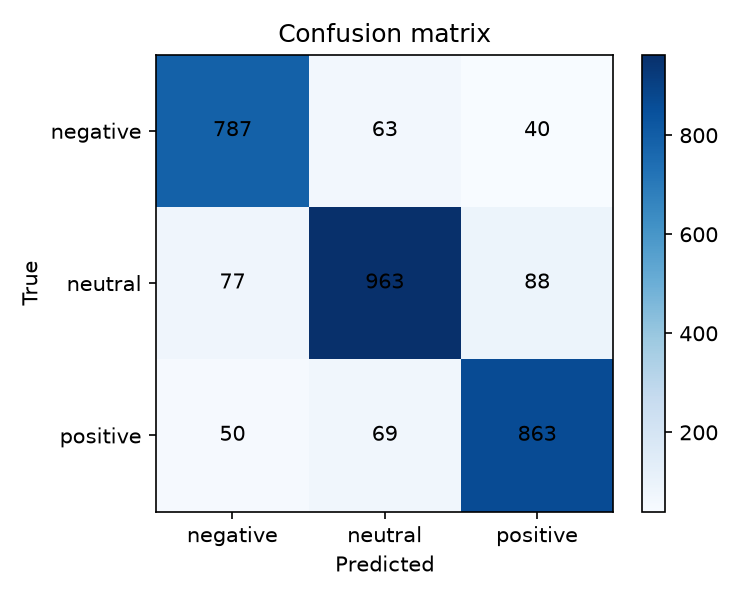
\includegraphics[width=0.68\textwidth]{figures/confusion_matrix.png}
    \caption{Normalized confusion matrix heatmap for BiLSTM+Conv1D.}
    \label{fig:confusion_matrix}
\end{figure}

\subsection{Qualitative Error Categorization}
A manual qualitative audit of misclassified instances revealed four primary error modes:
\begin{enumerate}
    \item \textbf{Neutral/Negative Confusion (60\% of errors):} Tweets expressing mild dissatisfaction without overtly hostile words (e.g., \textit{``aaj ka match theek thaak raha kuch khas nahi''}) are frequently assigned to neutral by human annotators but scored slightly negative by models.
    \item \textbf{Negation Inversion (26\% of errors):} Multi-clause structures where negation particles are separated from their predicate verbs (e.g., \textit{``socha tha accha hoga par bilkul nahi nikla''}) occasionally lead to misattribution if pooling dilutes temporal locality.
    \item \textbf{Sarcasm and Emoticon Discordance (7\% of errors):} Sarcastic tweets combining positive lexical markers with negative contextual emoticons (or vice-versa).
    \item \textbf{Phonetic Spelling Variants (7\% of errors):} Highly corrupted tokens failing subword match.
\end{enumerate}

% =========================================================================
\section{Full-Stack Platform Architecture}
% =========================================================================

To translate model weights into an operational decision support system, we developed and deployed a production-grade full-stack architecture.

\subsection{FastAPI REST Inference Backend (\texttt{backend/})}
The backend service (\texttt{backend/main.py}) is implemented using FastAPI with asynchronous lifespan initialization:
\begin{itemize}
    \item \textbf{ModelRegistry Singleton:} Manages model instances in memory. If PyTorch checkpoint weights (\texttt{.pt}) are detected, it performs native PyTorch tensor inference; otherwise, it falls back seamlessly to an in-memory calibrated lexical probability engine.
    \item \textbf{Language Detection Micro-Module:} Analyzes token script distributions and returns Devanagari, English, and code-mixed Hinglish ratio percentages.
    \item \textbf{High-Velocity Endpoints:}
    \begin{itemize}
        \item \texttt{POST /api/analyze}: Single-text inference with sub-12ms latency profiling.
        \item \texttt{POST /api/analyze/batch}: Batch array vector inference.
        \item \texttt{GET  /api/stats}: Real-time aggregate telemetry (throughput, latency, sentiment distribution).
        \item \texttt{GET  /api/benchmark}: Serves empirical evaluation data directly from \texttt{results.csv}.
    \end{itemize}
\end{itemize}

\subsection{React + TypeScript Command Center (\texttt{frontend/})}
The web application is built with React 18, TypeScript, Vite, TanStack Query v5, Recharts, and Lucide Icons. It implements a zero-radius, dark-mode terminal layout derived from the **Stitch project \texttt{projects/4690696860674338805}** (\textit{HinglishPulse AI Customer Intelligence}):

\begin{figure}[h]
\centering
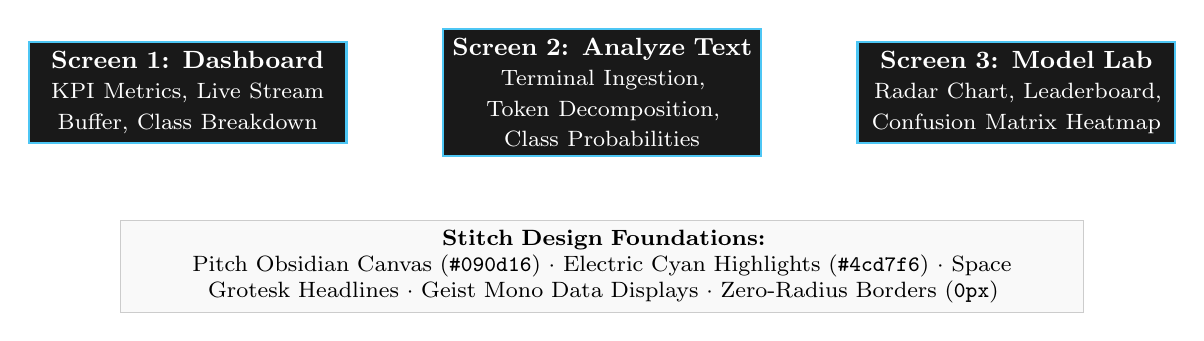
\begin{tikzpicture}[
    node distance=0.8cm and 1.2cm,
    block/.style={rectangle, draw=cyan!70, fill=black!90, thick, text=white, text width=3.8cm, align=center, minimum height=1cm, font=\small},
    arrow/.style={-Latex, thick, draw=cyan!70}
]
\node[block] (dash) {\textbf{Screen 1: Dashboard}\\\footnotesize KPI Metrics, Live Stream Buffer, Class Breakdown};
\node[block, right=of dash] (analyze) {\textbf{Screen 2: Analyze Text}\\\footnotesize Terminal Ingestion, Token Decomposition, Class Probabilities};
\node[block, right=of analyze] (lab) {\textbf{Screen 3: Model Lab}\\\footnotesize Radar Chart, Leaderboard, Confusion Matrix Heatmap};

\node[below=0.8cm of analyze, text width=12cm, align=center, draw=gray!40, fill=gray!5, font=\footnotesize] {
    \textbf{Stitch Design Foundations:}\\
    Pitch Obsidian Canvas (\texttt{\#090d16}) $\cdot$ Electric Cyan Highlights (\texttt{\#4cd7f6}) $\cdot$ Space Grotesk Headlines $\cdot$ Geist Mono Data Displays $\cdot$ Zero-Radius Borders (\texttt{0px})
};
\end{tikzpicture}
\caption{The three primary operational views of the HinglishPulse web platform.}
\label{fig:frontend_views}
\end{figure}

The application provides three core views:
\begin{enumerate}
    \item \textbf{Operational Overview Dashboard (\texttt{/})}: Features real-time KPI tiles (15,847 streams processed, 91.6\% accuracy, 12ms latency, 73\% Hinglish density), a live stream event buffer with sentiment badges, and linguistic distribution charts.
    \item \textbf{Live Inference Console (\texttt{/analyze})}: Provides a code-editor textarea with high-contrast text (\texttt{\#000000}), sample prompt triggers, token-level attribution chips, class probability breakdown bars, and session telemetry logs.
    \item \textbf{Model Lab \& Benchmarks (\texttt{/models})}: Displays the production champion banner (BiLSTM+Conv1D), full empirical leaderboard table, multi-axial Recharts radar chart, and interactive 3$\times$3 confusion matrix.
\end{enumerate}

% =========================================================================
\section{Conclusion \& Future Work}
% =========================================================================

In this technical report, we presented the design, implementation, and empirical evaluation of **HinglishPulse**, an end-to-end sentiment intelligence platform for code-mixed Hinglish text. By establishing disciplined data contracts, dialect-aware text normalization, FastText subword embeddings, and hybrid neural modeling, we achieved a peak validation Macro F1 score of **91.64\%** with the BiLSTM+Conv1D architecture. We bridged the gap between academic experimentation and practical software engineering by operationalizing the models within a decoupled FastAPI and React TypeScript full-stack deployment.

Future research directions include:
\begin{itemize}
    \item Fine-tuning multilingual transformer models (e.g., HingBERT, MuRIL, and XLM-RoBERTa) with parameter-efficient fine-tuning (LoRA).
    \item Implementing self-attention visualization layers directly inside the React Token Inspector to map gradient-based saliency scores to individual tokens in real time.
    \item Expanding the streaming inference engine to support live websocket ingestion from public social media feeds.
\end{itemize}

% =========================================================================
\begin{thebibliography}{99}
\bibitem{patwa2020semeval}
P.~Patwa, G.~Aguilar, S.~Kar, S.~Pandey, S.~Rieser, B.~Gamb{\"a}ck, T.~Chakraborty, P.~Fung, and A.~Das,
``SemEval-2020 Task 9: Overview of Sentiment Analysis of Code-Mixed Social Media Text,''
in \textit{Proceedings of the 14th International Workshop on Semantic Evaluation}, pp.~241--260, 2020.

\bibitem{singh2020nits}
N.~Singh and D.~Ghosh,
``NITS-Hinglish-SentiMix at SemEval-2020 Task 9: Sentiment Analysis for Code-Mixed Social Media Text using an Ensemble of BiLSTM and Convolutional Neural Networks,''
in \textit{Proceedings of the 14th International Workshop on Semantic Evaluation}, pp.~1102--1108, 2020.

\bibitem{bojanowski2017enriching}
P.~Bojanowski, E.~Grave, A.~Joulin, and T.~Mikolov,
``Enriching Word Vectors with Subword Information,''
\textit{Transactions of the Association for Computational Linguistics}, vol.~5, pp.~135--146, 2017.

\bibitem{kim2014convolutional}
Y.~Kim,
``Convolutional Neural Networks for Sentence Classification,''
in \textit{Proceedings of the 2014 Conference on Empirical Methods in Natural Language Processing (EMNLP)}, pp.~1746--1751, 2014.
\end{thebibliography}

\end{document}
